In this section, we will measure the curvature of two geometrical objects: a circle and a sinusoidal wave. The objective of this study is to find out how well our formulations of the normal unit vectors work by comparing the results to the analytical solutions we obtained in Sections \ref{sec:curvature_circle} and \ref{sec:curvature_sinusoidal_wave}. We will use the results of this section to later use the best formulations to minimize the curvature of the level set interface.

To measure curvature, we will integrate Equation \ref{eq:curvature_n} over the level set isocontour $\Gamma_{\phi=0}$ as follows:
%
\begin{equation}
	\centering
	\label{eq:curvature_integral}
	\int_{\phi=0} \kappa_{n} \,\mathrm{d}\Gamma = \int_{\phi=0} \Vert \frac{\mathrm{d}\mathbf{n}}{\mathrm{d}s} \Vert \,\mathrm{d}\Gamma
\end{equation}
%
% -----------------------------------------------------------------------------

\subsection{Sweep setup}
\label{sec:sweep_setup}

For our circle sweep, we will model the level set field with the following equation:
%
\begin{equation}
	\centering
	\label{eq:level_set_circle}
	\phi_{i} = r_{c} - \sqrt{x_{i} ^ 2 + y_{i} ^ 2}
\end{equation}
%
where $\phi_{i}$ represents a level set value at a node, and $x_{i}$ and $y_{i}$ are the spatial coordinates. We will vary the radius of the circle $r_{c}$ from a value of $0.25$ to $0.95$ in $100$ steps , as shown in Figure \ref{fig:circle_sweep_setup}. From equations \ref{eq:curvature_solution} and \ref{eq:curvature_integral}, the curvature will have a constant value of $2\pi$.
%
\begin{figure}[H]
	\centering
	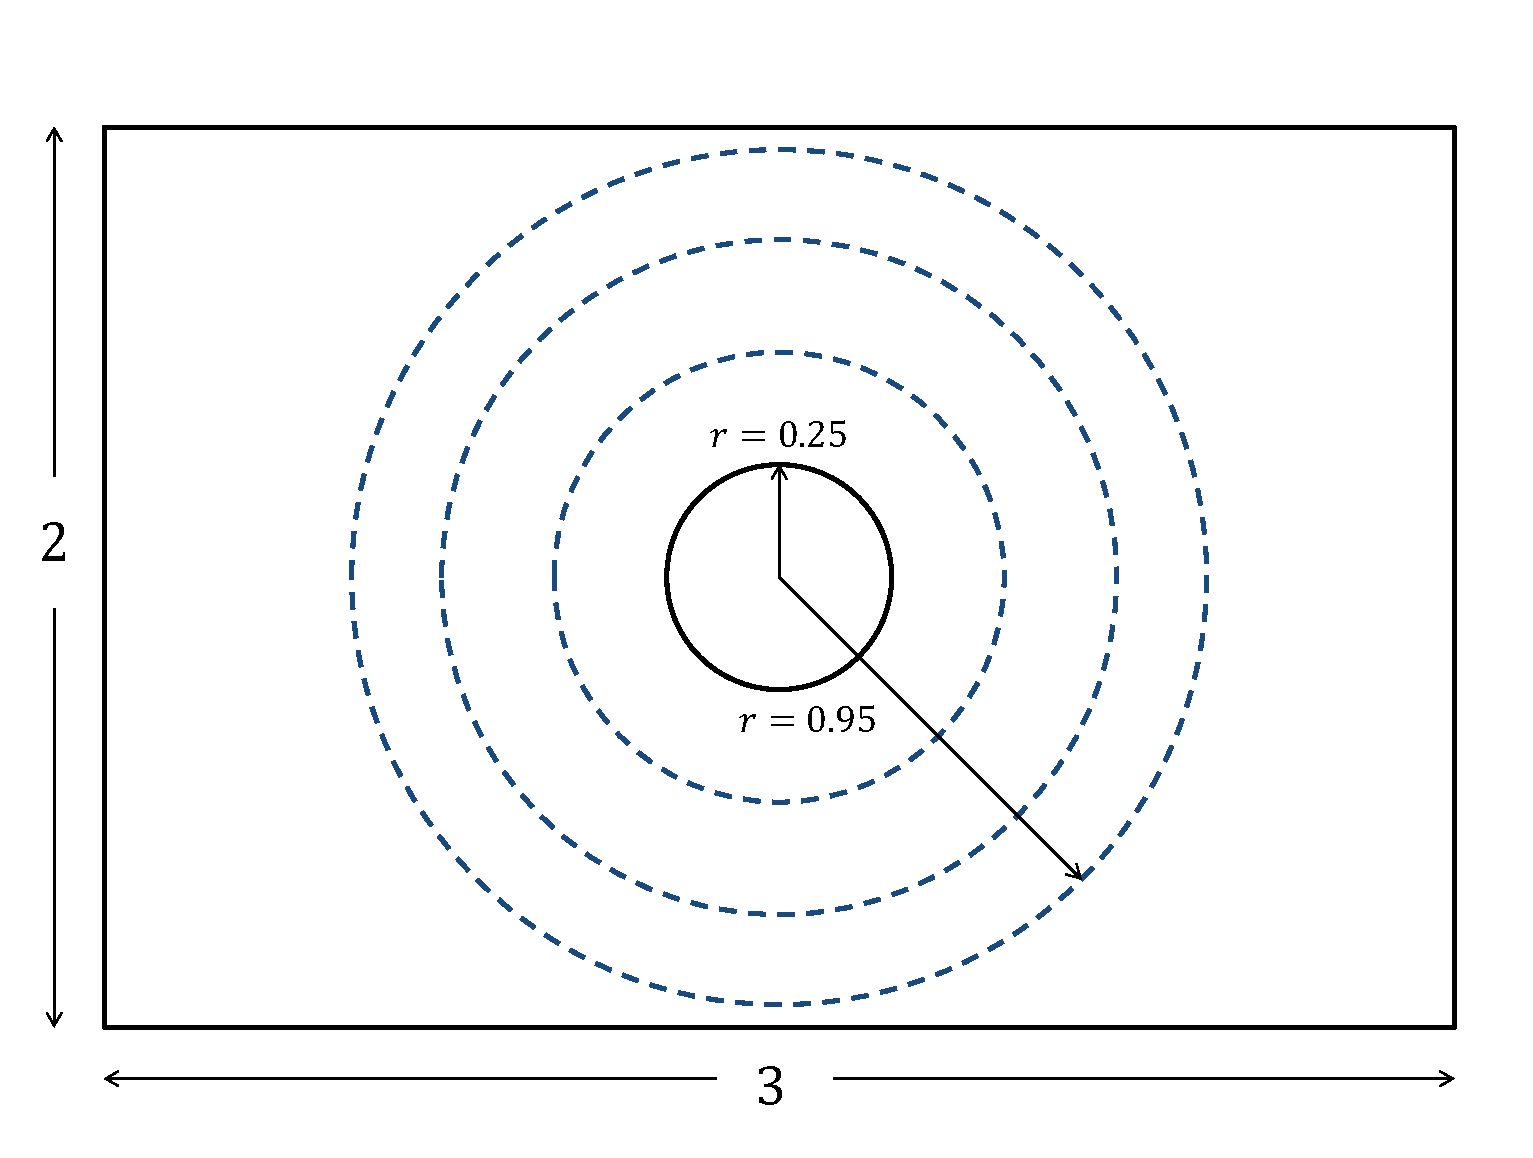
\includegraphics[scale=0.4]{circle_sweep_setup.eps}
	\caption{Setup for sweeping over the radius of a circle ranging from $0.25$ to $0.95$.}
	\label{fig:circle_sweep_setup}
\end{figure}

The sinusoidal wave will be modeled by the following equation:
%
\begin{equation}
	\centering
	\label{eq:level_set_sin_wave}
	\phi_{i} = y_{i} - A_{s} \sin \pi x_{i}
\end{equation}
%
where we will sweep over the amplitude of the sinusoidal wave, $A_{s}$, from $0.25$ to $0.75$. The value of the curvature for the sinusoidal wave cannot be computed analytically from Equation \ref{eq:sin_wave_curvature_solution}, so our approach will be to perform a mesh refinement study to ensure our equation converges to the right solution.
%
\begin{figure}[H]
	\centering
	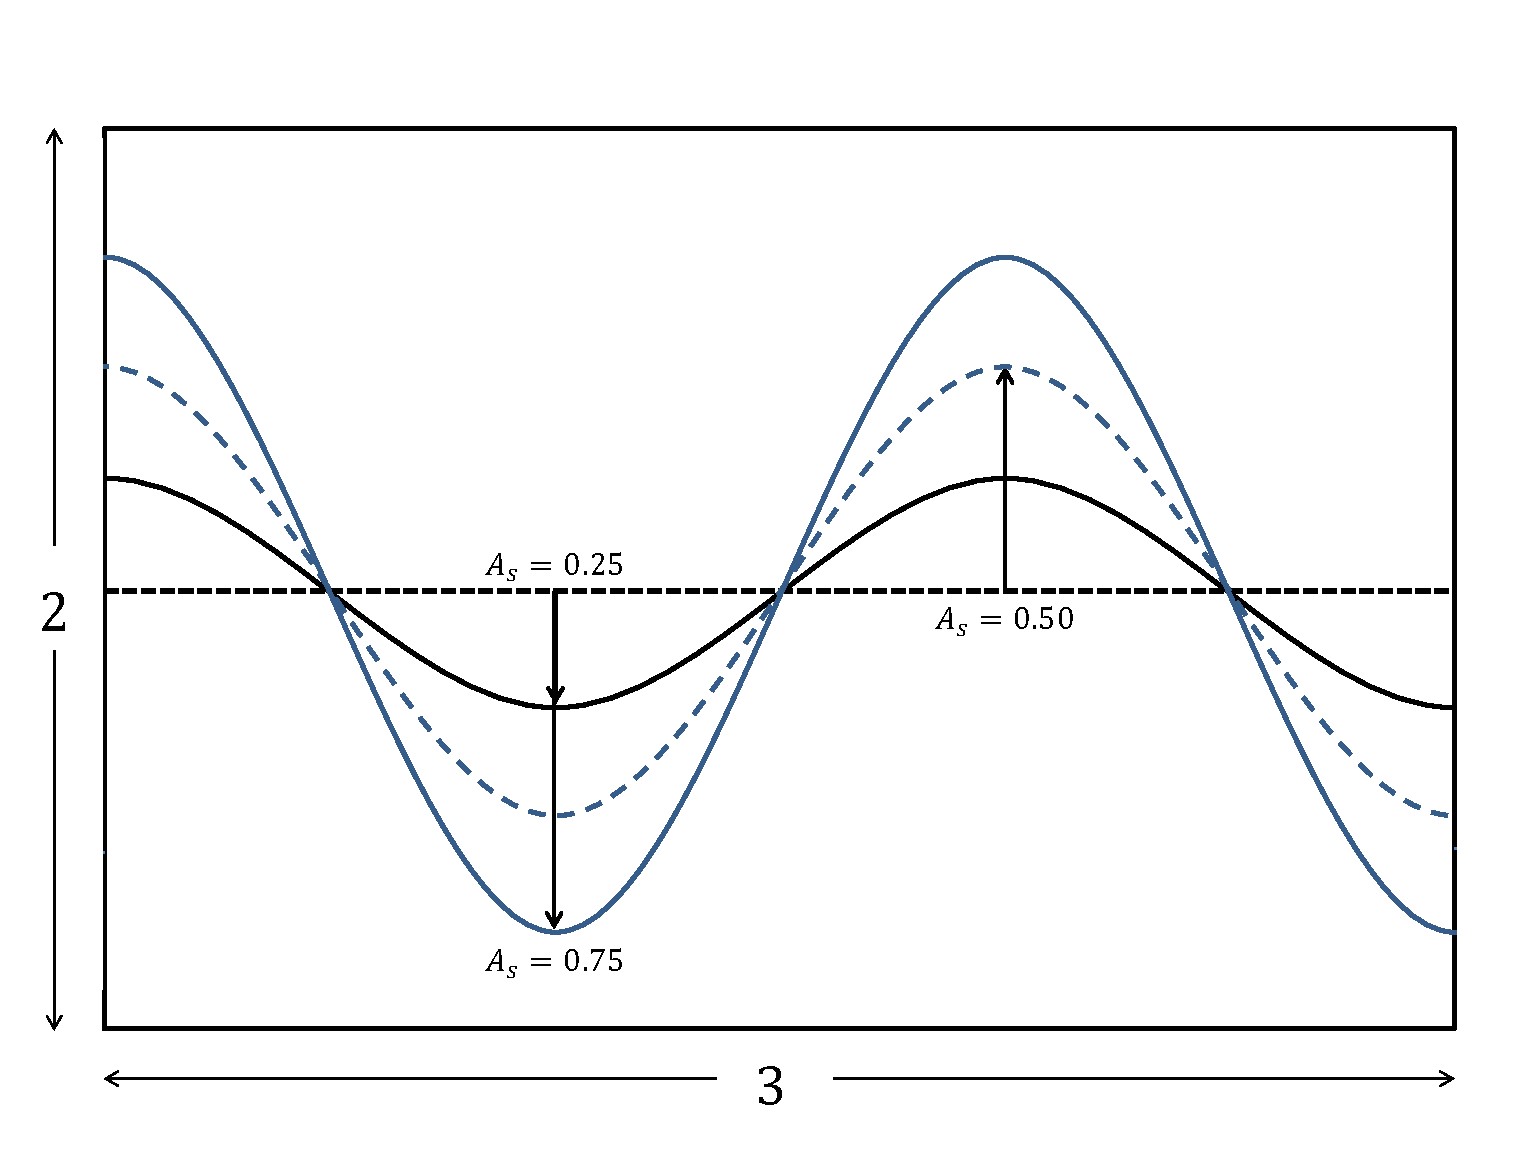
\includegraphics[scale=0.4]{sin_wave_sweep_setup.eps}
	\caption{Setup for sweeping over the amplitude of a sinusoidal wave ranging from $0.25$ to $0.75$.}
	\label{fig:sin_wave_sweep_setup}
\end{figure}
%
The mesh has spatial dimensions of $3L \times 2L$, and will be divided into $45 \times 30$ elements. The finer version of the mesh will have $180 \times 120$ elements.

% -----------------------------------------------------------------------------

\subsection{Sweep results}
\label{sec:sweep_results}

% -----------------------------------------------------------------------------

\subsubsection{$\mathbf{n}_{\phi}$ results}
\label{sec:nphi_results}

The results for the circular sweep with the $\mathbf{n}_{\phi}$ formulation and mesh $45 \times 30$ are shown in Figure \ref{fig:beam2D_quad4_XFEM_sweep_nphi_InterfaceCurvature_circle}. The absolute error between the analytical and numerical solutions is shown in Figure \ref{fig:beam2D_quad4_XFEM_sweep_nphi_InterfaceCurvature_circle_error}.
%
\begin{figure}[H]
	\centering
	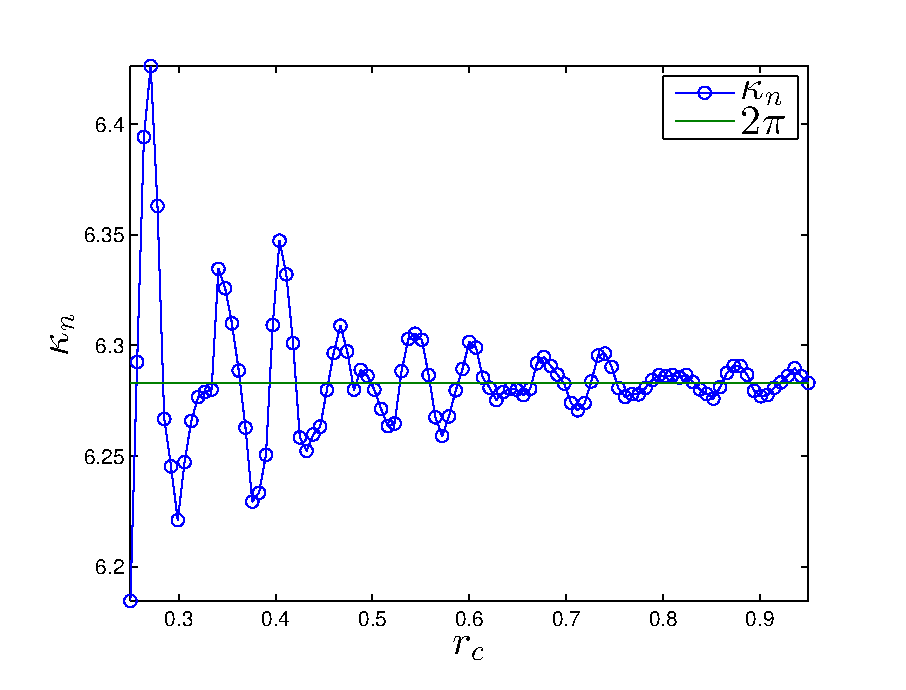
\includegraphics[scale=0.75]{beam2D_quad4_XFEM_sweep_nphi_InterfaceCurvature_circle.eps}
	\caption{Curvature for the circular sweep using the $\mathbf{n}_{\phi}$ formulation, with mesh $45 \times 30$.}
	\label{fig:beam2D_quad4_XFEM_sweep_nphi_InterfaceCurvature_circle}
\end{figure}
%
\begin{figure}[H]
	\centering
	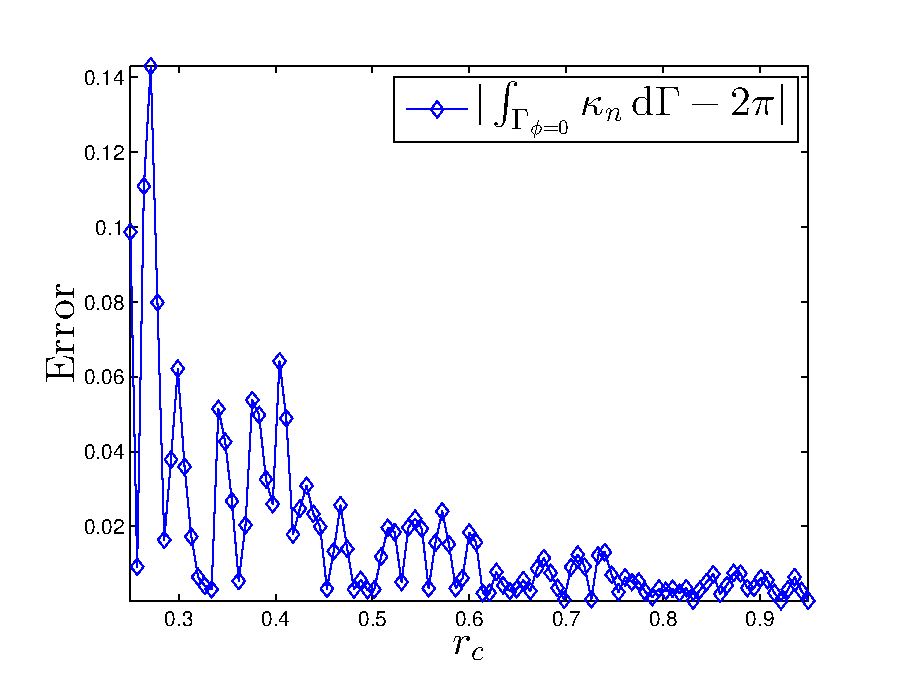
\includegraphics[scale=0.75]{beam2D_quad4_XFEM_sweep_nphi_InterfaceCurvature_circle_error.eps}
	\caption{Error in the curvature measure for the circular sweep using the $\mathbf{n}_{\phi}$ formulation, with mesh $45 \times 30$.}
	\label{fig:beam2D_quad4_XFEM_sweep_nphi_InterfaceCurvature_circle_error}
\end{figure}

The finer mesh results are shown in Figures \ref{fig:beam2D_quad4_XFEM_sweep_nphi_InterfaceCurvature_circle_finer} and \ref{fig:beam2D_quad4_XFEM_sweep_nphi_InterfaceCurvature_circle_finer_error}. The results confirm that as we refine the mesh, the solution approaches the value of $2\pi$.
%
\begin{figure}[H]
	\centering
	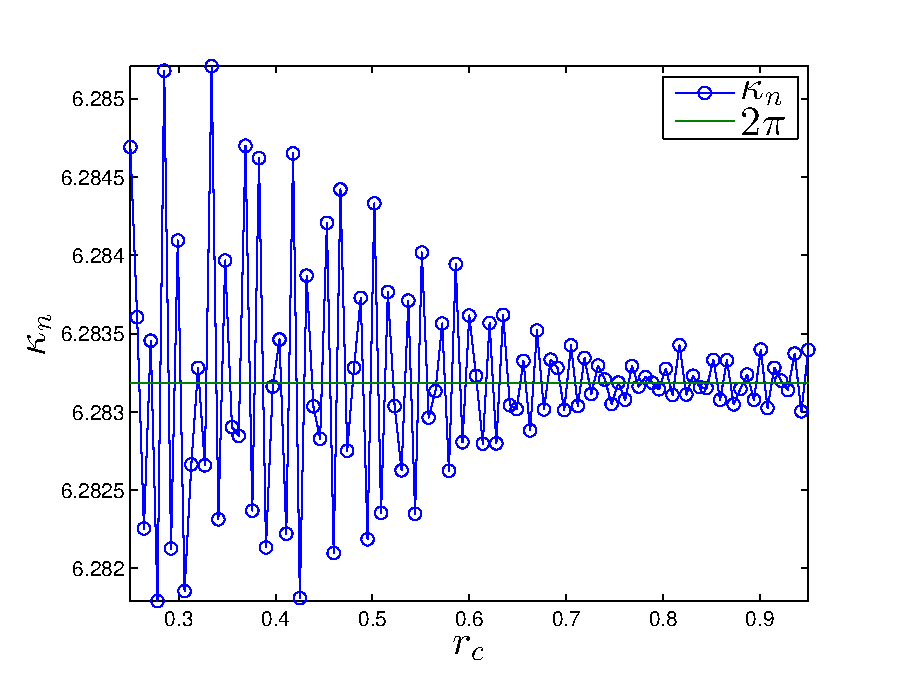
\includegraphics[scale=0.75]{beam2D_quad4_XFEM_sweep_nphi_InterfaceCurvature_circle_finer.eps}
	\caption{Curvature for the circular sweep using the $\mathbf{n}_{\phi}$ formulation, with mesh $180 \times 120$.}
	\label{fig:beam2D_quad4_XFEM_sweep_nphi_InterfaceCurvature_circle_finer}
\end{figure}
%
\begin{figure}[H]
	\centering
	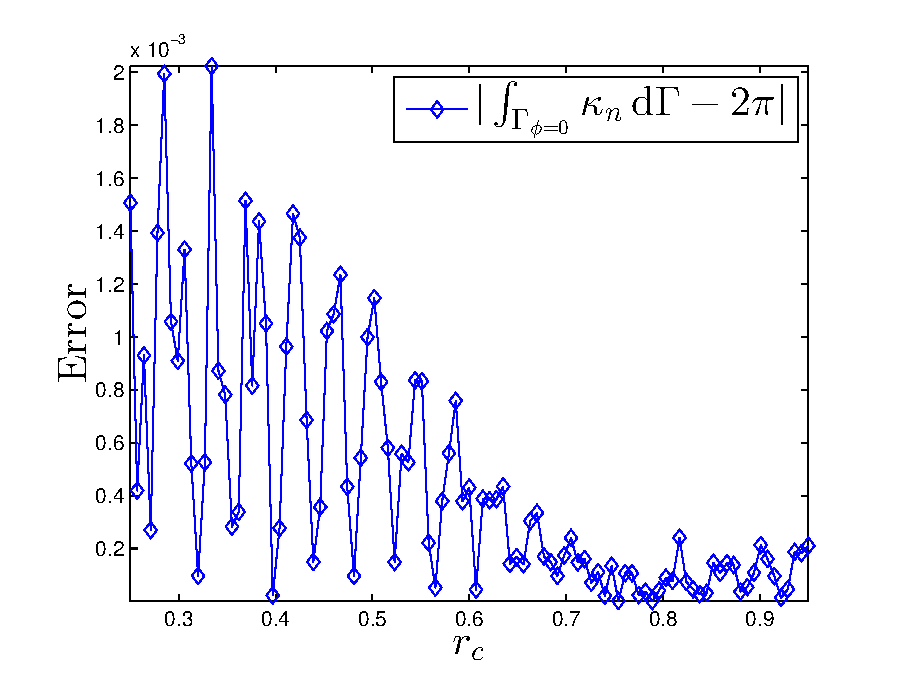
\includegraphics[scale=0.75]{beam2D_quad4_XFEM_sweep_nphi_InterfaceCurvature_circle_finer_error.eps}
	\caption{Error in the curvature measure for the circular sweep using the $\mathbf{n}_{\phi}$ formulation, with mesh $180 \times 120$.}
	\label{fig:beam2D_quad4_XFEM_sweep_nphi_InterfaceCurvature_circle_finer_error}
\end{figure}
%
% -----------------------------------------------------------------------------

\subsubsection{$\mathbf{n}_{u}$ results}
\label{sec:nnrm_results}

Using the $\mathbf{n}_{u}$ formulation, we get the results displayed in Figures \ref{fig:beam2D_quad4_XFEM_sweep_nnrm_InterfaceCurvature_circle} and \ref{fig:beam2D_quad4_XFEM_sweep_nnrm_InterfaceCurvature_sin} for a circle and sinusoidal wave, respectively. The error of the circular sweep compared to the analytical solution of Equation \ref{eq:curvature_solution} is shown in Figure \ref{fig:beam2D_quad4_XFEM_sweep_nnrm_InterfaceCurvature_circle_error}. The mesh size is $45 \times 30$. The scaling factor, $\gamma_{u}$, is 100.
%
\begin{figure}[H]
	\centering
	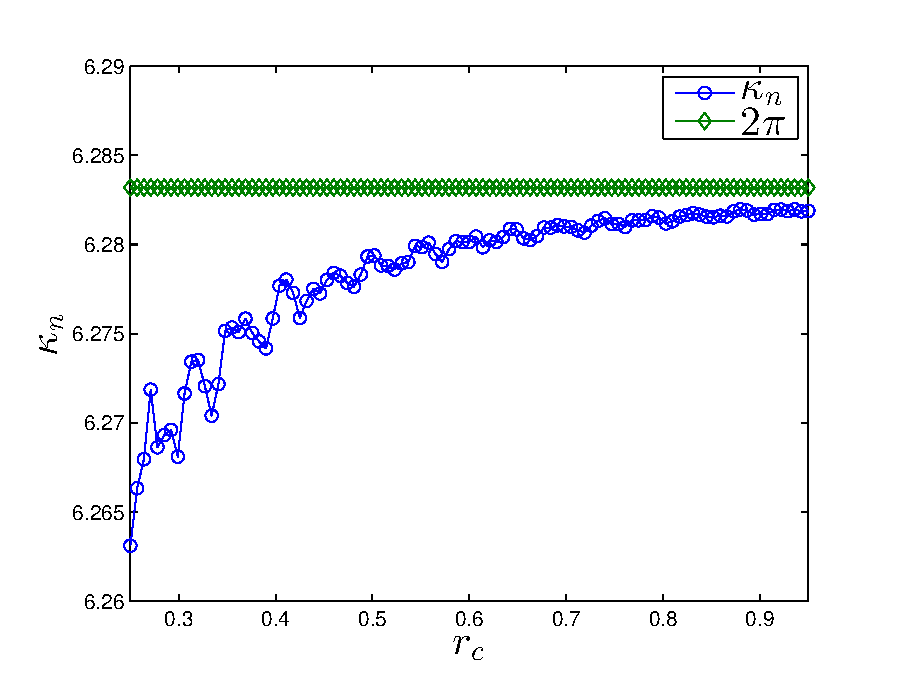
\includegraphics[scale=0.75]{beam2D_quad4_XFEM_sweep_nnrm_InterfaceCurvature_circle.eps}
	\caption{Curvature for the circular sweep using the $\mathbf{n}_{u}$ formulation, with mesh $45 \times 30$.}
	\label{fig:beam2D_quad4_XFEM_sweep_nnrm_InterfaceCurvature_circle}
\end{figure}
%
\begin{figure}[H]
	\centering
	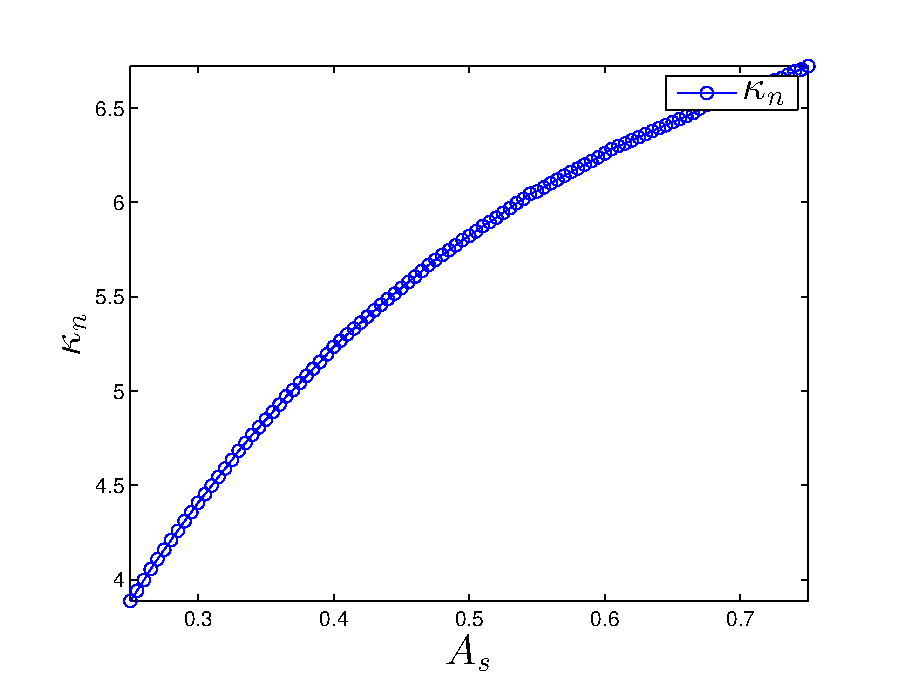
\includegraphics[scale=0.75]{beam2D_quad4_XFEM_sweep_nnrm_InterfaceCurvature_sin.eps}
	\caption{Curvature for the sinusoidal wave sweep using the $\mathbf{n}_{u}$ formulation, with mesh $45 \times 30$.}
	\label{fig:beam2D_quad4_XFEM_sweep_nnrm_InterfaceCurvature_sin}
\end{figure}
%
\begin{figure}[H]
	\centering
	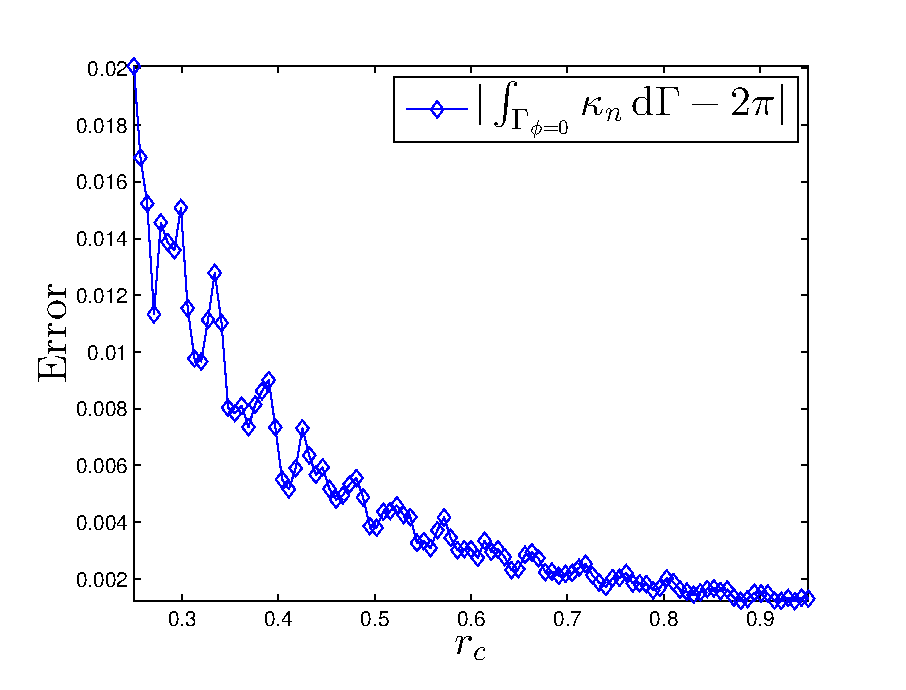
\includegraphics[scale=0.75]{beam2D_quad4_XFEM_sweep_nnrm_InterfaceCurvature_circle_error.eps}
	\caption{Error in the curvature measure for the circular sweep using the $\mathbf{n}_{u}$ formulation, with mesh $45 \times 30$.}
	\label{fig:beam2D_quad4_XFEM_sweep_nnrm_InterfaceCurvature_circle_error}
\end{figure}
%
% -----------------------------------------------------------------------------

\subsubsection{$\mathbf{n}_{\psi}$ results}
\label{sec:npsi_results}

Measuring the curvature using the $\mathbf{n}_{\psi}$ formulation requires us to define the parameter $\epsilon$. We will examine the influence of $\epsilon = 1.0$, $\epsilon = 2.0$, and $\epsilon = 4.0$, and the benefits of using $\nabla \psi = \frac{\partial \psi}{\partial \mathbf{x}}$ or 
$\nabla \psi = \frac{\partial \psi}{\partial \phi} \frac{\partial \phi}{\partial \mathbf{x}}$.

% -----------------------------------------------------------------------------

\subsubsection{Conclusions of the sweep study}
\label{sec:sweep_study_conclusions}

Figures \ref{fig:beam2D_quad4_XFEM_sweep_nphi_InterfaceCurvature_circle} and \ref{fig:beam2D_quad4_XFEM_sweep_nphi_InterfaceCurvature_circle_finer} show measuring the curvature by using $\mathbf{n}_{\phi}$ causes oscillations that are not resolved by refining the mesh. Using a projection scheme in the $\mathbf{n}_{u}$ and $\mathbf{n}_{\psi}$ formulations yields a smoother curvature measure than solving for the normal unit vector in the strong form; however, oscillations still exist, although to a lower degree.